\documentclass{article}
\usepackage{tikz}
\usetikzlibrary{matrix}

\begin{document}

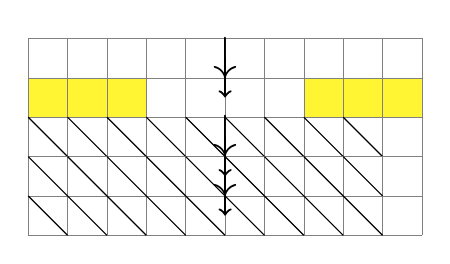
\begin{tikzpicture}[scale=0.5]
    % Define the grid for the first row
    \draw[help lines] (0,0) grid (10,2);
    
    % Draw the second row with yellow shaded cells
    \fill[yellow!80!white] (0,0) rectangle (3,1);
    \fill[yellow!80!white] (7,0) rectangle (10,1);
    \draw[help lines] (0,0) grid (10,1);
    
    % Draw the third row with diagonal lines
    \draw[help lines] (0,-1) grid (10,0);
    \foreach \x in {1,...,9} {
        \draw (\x,-1) -- (\x-1,0);
    }
    
    % Draw the fourth row with diagonal lines
    \draw[help lines] (0,-2) grid (10,-1);
    \foreach \x in {1,...,9} {
        \draw (\x,-2) -- (\x-1,-1);
    }
    
    % Draw the fifth row with diagonal lines
    \draw[help lines] (0,-3) grid (10,-2);
    \foreach \x in {1,...,9} {
        \draw (\x,-3) -- (\x-1,-2);
    }
    
    % Draw the arrow between rows
    \draw[->,thick] (5,1.5) -- (5,0.5);
    \draw[->,thick] (5,-0.5) -- (5,-1.5);
    \draw[->,thick] (5,-1.5) -- (5,-2.5);
    
    % Add labels to indicate the states
    \node at (5,1.5) {\textbf{\LARGE $\downarrow$}};
    \node at (5,-0.5) {\textbf{\LARGE $\downarrow$}};
    \node at (5,-1.5) {\textbf{\LARGE $\downarrow$}};
\end{tikzpicture}

\end{document}